% GwenLaya v4 paper. Every number in this file is read from one of:
%   papers/numbers_v4.json, papers/tables_v4.tex (both written by scripts/analyze_study.py),
%   docs/RESULTS_VERDICT.md, docs/DEVIATIONS.md, docs/FREEZE_ADDENDUM_NIGHT_2026-10-07.md,
%   docs/STAGE_LOG.md, results/results_n257_l4_gpu.json, results/results_n60_cpu.json,
%   /mnt/data/home/xavkal/gwaya-data/spend_ledger.jsonl,
%   /mnt/data/home/xavkal/gwaya-data/night/results/L0_env.json,
%   gs://socrateai-datalake-gen-lang-client-0625573011/gwenlaya_v4/tpu_smoke/gwenlaya-tpu-smoke-215529/.
% Unknown values are written TBD.
\documentclass[11pt,a4paper]{article}
\usepackage[margin=2.4cm]{geometry}
\usepackage[T1]{fontenc}
\usepackage[utf8]{inputenc}
\usepackage{lmodern}
\usepackage{amsmath,amssymb}
\usepackage{booktabs,array,longtable}
\usepackage{graphicx}
\usepackage{pdflscape}
\usepackage{enumitem}
\usepackage{xcolor}
\PassOptionsToPackage{hyphens}{url}
\usepackage[hidelinks]{hyperref}
\usepackage{url}
\usepackage{seqsplit}
\Urlmuskip=0mu plus 1mu
\makeatletter\g@addto@macro{\UrlBreaks}{\do\-\do\_}\makeatother
\setlength{\emergencystretch}{3em}\sloppy
\setlist{itemsep=2pt,topsep=4pt}
\graphicspath{{figures_v4/}}
\newcommand{\TBD}{\textsf{TBD}}
\newcommand{\code}[1]{\texttt{\detokenize{#1}}}

\title{GwenLaya v4: a pre-registered study of answering only when a check can back the answer\\[4pt]
\large Interim report after the first night run: registered design, deviations,\\
one descriptive single-arm result, and no completed pre-registered test}
\author{Xavier Callens\\AutoevolveAI / ANSE open-source project}
\date{8 October 2026 \quad (draft v4.0, branch \texttt{night/2026-10-07})}

\begin{document}
\maketitle

\begin{abstract}
GwenLaya is a system design in which a small open model (Qwen3.5 family) answers a programming or
mathematics question only when an executed check or a calibrated confidence score supports the
answer, and otherwise abstains or escalates to a larger tier. We pre-registered fifteen hypotheses
(two primary: fewer confident-wrong answers than log-probability selective prediction at matched
coverage, H1; lower cost per correct answered item than always using the largest tier with the
gate, H3) before any GwenLaya run. This report covers the first, budget-limited night run.
\textbf{No pre-registered hypothesis test was completed.} The only scored data are 80 items from
one arm that is not a registered arm (Qwen3.5-2B, q4\_K\_M, CPU, no gate, no calibrator). On those
items accuracy was 0.175 (95\% cluster bootstrap CI 0.10--0.25), and the raw
$\exp(\text{mean log-prob})$ confidence was badly calibrated (ECE 0.700) and only weakly
informative (AUROC 0.618, CI 0.422--0.811). These are descriptive numbers, not tests. The math
part of them is invalid because of a prompt-path defect we found after generation, and the Rust
part is unvalidated. The one systems claim that could be checked, the budget (H13), holds on an
interim basis. We also report a TPU feasibility finding (Qwen2.5 generation works on a v5e chip
via vLLM's TPU build; Qwen3.5 did not load in time; no TPU LoRA path was found for Qwen3.5 dense
or Qwen3.8), the GCP spend actually recorded, and every deviation from the registration. We
begin by restating the retraction of a v3 claim and the failed v3 gate.
\end{abstract}

%-----------------------------------------------------------------------------
\section{Retraction and the v3 gate failure, stated first}\label{sec:retraction}

\paragraph{Retraction.} Revision 3.1.0 of the predecessor report~\cite{gwayav3} claimed that the
low-tier optimizer improved pass rates by at least $+8.0$ percentage points. That claim rested on a
hand-written results file with invented numbers (A0 33\,\%, A3 100\,\%). The file was fabricated, it
has been deleted, and it is not evidence (\code{results/PREREGISTRATION.md}). The claim is
retracted. Nothing in this paper depends on it.

\paragraph{The measured v3 gate failed.} The pre-registered v3 gate was
$\text{A3}-\text{A0}\ge +8.0$ points pass@1 on MBPP-sanitized with \code{qwen2.5-coder:1.5b}. Both
measured runs \textbf{FAIL} that gate:
\begin{itemize}
\item $n=60$, CPU: A3$-$A0 $=+6.67$ points, 95\% CI $[1.67, 13.33]$, 4 gained / 0 lost, exact
  McNemar $p=0.125$; verdict FAIL (\code{results/results_n60_cpu.json}).
\item $n=257$, L4 GPU: A0 64.2\,\%, A3 71.98\,\%, A3$-$A0 $=+7.78$ points, 95\% CI $[4.67, 11.28]$,
  20 gained / 0 lost; verdict FAIL against $+8.0$. This file's \code{git_commit} field is empty
  (\code{results/results_n257_l4_gpu.json}).
\end{itemize}
The improvement is real in the sense that the CI excludes zero, but it misses the registered
threshold, and we report it as a FAIL. The same file shows the v3 gate's weakness that motivates
v4: of answers the gate called VERIFIED (coverage 80.93\,\%), only 88.94\,\% passed the hidden
tests. By arithmetic on those two file values (not a measurement), about 8.95\,\% of all problems
were confident-wrong under v3.

%-----------------------------------------------------------------------------
\section{What GwenLaya is and what was registered}\label{sec:design}

The full registration is \code{docs/GWENLAYA_PREREGISTRATION.md} (revision 2, design freeze; sha256
of each revision in \code{docs/PREREG_FREEZE.txt}). In brief:

\begin{itemize}
\item \textbf{System (GL).} Generate with a small Qwen3.5 tier; run a \emph{gate-visible} executed
  check that never sees the scoring tests; score the candidate with a calibrated confidence head
  (a LoRA head on the \code{convaiinnovations/laya} encoder); answer VERIFIED, LIKELY\_CORRECT($p$),
  abstain, or escalate to a larger tier. The label for calibration is the outcome on the
  \emph{hidden} checks, so VERIFIED is never treated as ground truth.
\item \textbf{Eval pool E.} HumanEval+ and MBPP+~\cite{evalplus} (Python, 542 items), MultiPL-E
  Rust~\cite{multiple} (510), MATH-500~\cite{math,letsverify} (500), and miniF2F Lean 4 (244,
  outside the pooled analysis).
\item \textbf{Arms.} B1 smallest tier alone; B2 largest tier alone; B3 log-probability selective
  prediction~\cite{selective}; B4 self-consistency; B5 largest tier with the v3-style gate only;
  B6 Laya zero-shot; LR and a shuffled-label negative control SH.
\item \textbf{Primary family} (Holm~\cite{holm}, $m=2$): H1, CWR(GL)$-$CWR(B3) at matched coverage,
  exact one-sided McNemar~\cite{mcnemar} plus a cluster-stratified paired bootstrap, MEI 3.0 points;
  H3, cost per correct answered item, GL vs B5, MEI 25\,\% reduction, with answered accuracy
  non-inferior by 2.0 points.
\item \textbf{Secondary:} calibration (H4 ECE~\cite{guo}, H5 Laya vs LR AUROC, H6 split-conformal
  selective error~\cite{conformal}); quantization (H8); training (H9); systems (H13 budget, H14
  endpoint latency, H15 preemption). \textbf{Exploratory:} H2, H7, H10--H12.
\end{itemize}
Hypothesis wording, metrics, MEIs and decision rules have not been changed.

%-----------------------------------------------------------------------------
\section{The night run and its deviations}\label{sec:deviations}

The night of 2026-10-07/08 was meant to run the primaries cheaply. Two constraints shaped it:
the total GCP budget (\$50 hard, \$45 working ceiling for this programme, \$40 planned), and the
fact that the project's only GPU quota unit (\code{GPUS_ALL_REGIONS} limit 1) was held all night by
a VM that is not part of this project and that we did not touch. All generation therefore ran on a
shared 8-core CPU, and the scope was cut. Every cut is in \code{docs/DEVIATIONS.md}, was written
before the run it affects, and is summarised in Table~\ref{tab:dev}.

\begin{table}[t]\centering\footnotesize\setlength{\tabcolsep}{4pt}
\caption{Deviations from the registration for the night run (from \code{docs/DEVIATIONS.md}). Reason codes: B = budget, G = no GPU slot, T = CPU wall clock, I = implementation or defect.}
\label{tab:dev}
\begin{tabular}{l p{4.6cm} p{6.0cm} p{2.2cm}}\toprule
\# & Registered & Night run & Why\\\midrule
D1 & E = 1,552 items on L4 & E-night: seeded prefix, 80 items (python 28, rust 26, math 26) & G, T\\
D2 & tiers 2B/4B/9B/27B & 2B and 4B only (B2/B3/B5 on 4B) & G, T\\
D3 & H3 cost in L4 GPU-seconds & CPU-seconds on this machine & G\\
D4 & separate calibration set C & 5-fold cross-fitting on E-night by source cluster & T; C was not label-matched\\
D5 & Laya LoRA r=16 heads & LoRA only if CPU timing fits, else frozen-embedding probe & T\\
D6 & llama.cpp server & llama.cpp b11476 CPU; Ollama not used (no logprobs) & I\\
D7 & Lean 4 (E, C, H11) & dropped tonight & T, B\\
D8 & SFT, DPO, S4b--S5 & deferred; H9 deferred, H10--H12 dropped & G, B\\
D9 & B4 self-consistency, second seed & dropped & B, T\\
D10 & GSM8K, AIME25, LiveCodeBench, MBPP anchor, 0.8B & dropped & B, T\\
D11 & H8 on full E & 300-item 9B subsample only if GPU; no TOST & G\\
D12 & endpoint, 4--6 cold samples & 4 samples, only after G1 & G, B\\
D14--D15 & \code{-t 8}; 256-token tok/s probe & \code{-t 4}; 64 tokens & T (foreign CPU load)\\
D16 & -- & fix: multi-letter words in math checker return undecided & I\\
D17 & reference passes its own checks & Rust: typecheck only (no reference solution) & I\\
D18 & decontaminate T, C & all 170 MBPP-sanitized calib items removed; no T/C & I\\
D19 & n from measured throughput & n from measured tok/s and an \emph{assumed} 196.6 tokens/item & T\\
D20 & prompt text not fixed & gate-visible tests and prompts frozen in the task file & I\\
D21 & -- & logprobs and per-call CPU-seconds captured & I\\
D22 & \code{random.Random(0)} bootstrap & numpy \code{default_rng(0)}, 10,000 resamples & I\\
D23 & -- & scored the 80 L2 generations; single-arm descriptives added & I\\
\bottomrule\end{tabular}\end{table}

\paragraph{Benchmarks reduced.} To stay within budget and wall clock we ran no benchmark beyond the
three primary domains, on 80 of their 1,541 included items, with two tiers instead of four. Lean 4,
GSM8K, AIME25, LiveCodeBench, the MBPP continuity anchor, the 0.8B tier, self-consistency and the
second seed were dropped (D7--D10). The registered design for all of them stays in the
registration and is not reported here as if it had run.

\paragraph{Power was known to be insufficient before generation.} The freeze addendum computed the
power of H1's exact McNemar test at $n=80$ before any item was generated: 0.052 at the 3-point MEI
and 0.261 at a 6-point effect ($\alpha=0.025$). A non-significant H1 at this $n$ would therefore
have been inconclusive, not evidence of no effect.

\paragraph{What actually ran.} L0 (environment, throughput), L1 (manifest, freeze addendum,
decontamination), L2 (2B generation on all 80 E-night items, 72 minutes wall), and scoring of those
80 generations. L3 (4B generation) was held because the L2 review found a blocking defect
(Section~\ref{sec:defects}). G1 (GPU) and E1 (endpoint) never ran: the GPU slot never freed. No
Laya head, calibrator, threshold or second arm exists.

%-----------------------------------------------------------------------------
\section{Results}\label{sec:results}

\subsection{Per-hypothesis verdicts}

Table~\ref{tab:verdict} reproduces \code{docs/RESULTS_VERDICT.md}. For every hypothesis that did
not run, the probability column is the \textbf{red-team prior} written in the review before the run
(\code{docs/PROPOSAL_REVIEW.md}, copied into \code{docs/DEVIATIONS.md}). It is \emph{not} an
estimate from data. Only H13 has a probability that reflects an executed check.

\begin{table}[t]\centering\small
\caption{Verdicts after the night run. ``Prior'' = red-team prior that the hypothesis would be supported, written before any data; not updated by evidence.}
\label{tab:verdict}
\begin{tabular}{l l l l p{6.3cm}}\toprule
H & Role & Verdict & $P(\text{true})$ & Basis\\\midrule
H1 & primary & not run & 0.45 (prior) & no GL or B3 arm; power at MEI with $n=80$ was 0.05\\
H3 & primary & not run & 0.50 (prior) & no GL or B5 arm; cost unit would be CPU-s (D3)\\
H4 & secondary & not run & 0.15 (prior) & no cross-fitted scores; no Laya head\\
H5 & secondary & not run & 0.25 (prior) & same\\
H6 & secondary & not run & 0.40 (prior) & same\\
H8 & secondary & not run & 0.30 (prior) & needs GPU (D11)\\
H9 & secondary & deferred & 0.25 (prior) & D8\\
H13 & systems & supported (interim) & 0.97 & deterministic ledger check, Sec.~\ref{sec:spend}\\
H14 & systems & not run & 0.50 (prior) & needs E1, which needs the GPU (D12)\\
H15 & systems & not run & 0.70 (prior) & offline test is not the registered SIGKILL check\\
H2 & exploratory & not run & 0.08 (prior) & no GL or B5 arm\\
H7 & exploratory & not run & 0.10 (prior) & gate field is null in every scored row\\
H10 & exploratory & dropped & 0.05 (prior) & D8\\
H11 & exploratory & dropped & 0.12 (prior) & D7, D8\\
H12 & exploratory & dropped & 0.12 (prior) & D8\\
\bottomrule\end{tabular}\end{table}

\paragraph{H13 (budget).} Decision rule: ledger total $\le\$40$ planned and $\le\$50$ hard, and no
stage over $1.25\times$ its cap twice. The ledger has 3 lines with a known USD total of 0.0 and 2
unpriced lines (2,706 seconds of TPU time). With the \textasciitilde\$0.84 estimate for those lines
(Section~\ref{sec:spend}) the rule holds with a wide margin, and no stage has spent anything against
its cap. The 0.97 is not a bootstrap: the check is deterministic, and the remaining 0.03 covers the
unpriced lines, the fact that the planned GCS ledger \code{runs/LEDGER.jsonl} does not exist, and
spend in later nights. H13 is a whole-study claim, so this verdict is interim.

\paragraph{H15 (preemption).} \code{tests/test_run_study.py::test_resume_after_kill_mid_run}
passes, but it simulates a death by appending a torn line; it sends no SIGKILL and measures no lost
wall time. It is weak support that resume is item-granular, not the registered verification, so the
probability stays at the prior.

\subsection{Descriptive single-arm result (not a pre-registered test)}

The scored arm \code{base} is Qwen3.5-2B q4\_K\_M on llama.cpp~\cite{llamacpp}, greedy, thinking off,
\code{max_new_tokens} 1024, with no gate, no calibrator and no escalation. It is not one of the
registered arms. Confidence is the raw $\exp(\text{mean token log-prob})$, uncalibrated and not
cross-fitted. Intervals are 95\% cluster-stratified bootstrap percentile intervals (10,000
resamples, seed 0). The machine-generated tables of \code{scripts/analyze_study.py}
(generation descriptives, the arm table and the script's own hypothesis status) are reproduced
unedited in Appendix~\ref{app:tables}. Accuracy was 0.175 (CI 0.10--0.25) and coverage 1.0;
the confident-wrong rate was 0.825 (CI 0.75--0.90), an upper bound because every UNVERIFIED answer
is counted as wrong.

\begin{table}[t]\centering\small
\caption{Calibration and selective-prediction metrics for the raw confidence of arm \code{base} (from \code{papers/numbers_v4.json}; $n=80$).}
\label{tab:calib}
\begin{tabular}{lcc}\toprule
Metric & Point & 95\% CI\\\midrule
ECE & 0.700 & 0.626--0.771\\
Brier & 0.630 & 0.571--0.686\\
AUROC & 0.618 & 0.422--0.811\\
AURC & 0.716 & 0.586--0.859\\
Cost per correct (server CPU-s) & 1178 & 732--2114\\
\bottomrule\end{tabular}\end{table}

\begin{figure}[t]\centering
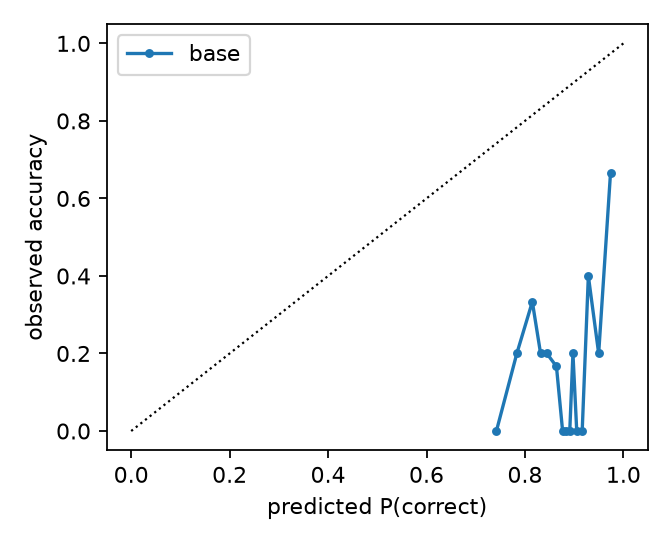
\includegraphics[width=0.46\linewidth]{reliability.png}\hfill
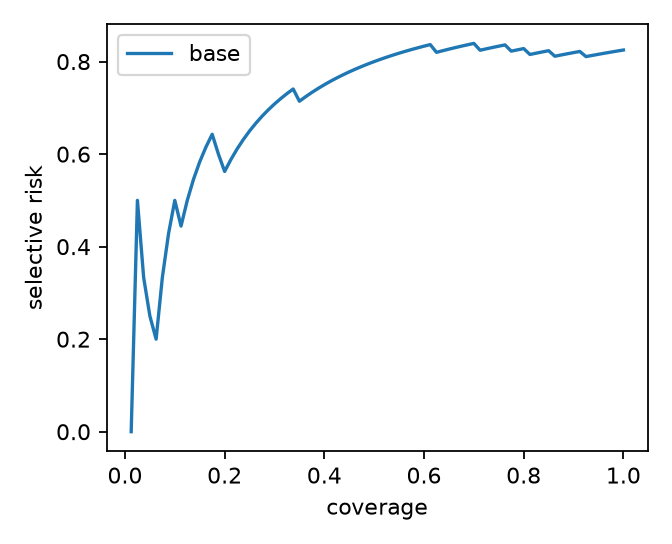
\includegraphics[width=0.46\linewidth]{risk_coverage.png}
\caption{Arm \code{base}, raw confidence, $n=80$. Left: reliability diagram. Right: risk--coverage
curve. Descriptive only; not cross-fitted; the math items in it are invalid (Section~\ref{sec:defects}).}
\label{fig:calib}
\end{figure}

Per domain (counted from \code{rows.jsonl} in \code{docs/RESULTS_VERDICT.md}): Python 11 VERIFIED
/ 17 FAILED; Rust 0 VERIFIED / 13 FAILED / 13 UNVERIFIED; Math 3 VERIFIED / 18 FAILED / 5
UNVERIFIED. Pooled accuracy 0.175 is therefore driven by Python (11 of the 14 correct items).

What we read from this, and no more: the raw log-probability of a 2B model at q4 is concentrated
near 1 while accuracy is near 0.2 (Figure~\ref{fig:calib}), so it is not a usable confidence
without calibration, and its AUROC interval includes 0.5. This is consistent with the motivation
for a calibrated head, but it does not test H1, H4 or H5.

\subsection{Defects found, and why some numbers are invalid}\label{sec:defects}

\begin{enumerate}
\item \textbf{Math prompt path (blocking).} All 26 math completions were produced with the Python
  code system prompt and a \verb|```python| prefill, because the prompt builder falls back to the
  \code{python} tag for any domain it does not list. 0 of 26 contain \verb|\boxed|. The frozen user
  prompt asked for a boxed answer, but the system prompt and prefill overrode it. The 3/26 math
  VERIFIED says nothing about the model's math ability. The fix (math system prompt, no code
  prefill) and a regeneration of the 26 items must be logged as a new deviation before any rerun;
  neither has happened yet.
\item \textbf{Rust harness unvalidated.} MultiPL-E has no reference solutions, so the Rust harness
  was checked only by typechecking test bodies (D17). 0/26 VERIFIED with 13/26 UNVERIFIED is as
  consistent with a harness or toolchain problem as with model weakness. Until one known-good Rust
  program passes end to end, the Rust rate is unverified.
\item \textbf{Gate not recorded.} The \code{gate} field is null in every scored row, so VERIFIED
  precision against hidden checks (H7) cannot be computed from this run.
\end{enumerate}

\paragraph{Meaning of ``verified'' in this paper.} An item is VERIFIED only if it passed the named
executed checks: for Python, the full EvalPlus test suite run in a bubblewrap sandbox; for Rust,
compilation and all \code{assert_eq!} lines of the MultiPL-E test with \code{rustc}; for math, a
sympy/numeric equivalence check against the gold answer. It means nothing more. It does not mean
the solution is correct on other inputs, and for Rust the harness itself is not yet validated.

%-----------------------------------------------------------------------------
\section{TPU feasibility finding}\label{sec:tpu}

Because the GPU slot was unavailable, we tested whether a Cloud TPU v5e could replace it. Two
smoke runs were made on a single-chip v5litepod-1 (logs under
\url{gs://socrateai-datalake-gen-lang-client-0625573011/gwenlaya_v4/tpu_smoke/gwenlaya-tpu-smoke-215529/}).
The first, on a spot VM, was preempted after about 4 minutes with no results. The second, on demand:

\begin{itemize}
\item \textbf{Qwen2.5 works.} \code{Qwen/Qwen2.5-Coder-1.5B-Instruct} loaded and generated with
  vLLM~\cite{vllm} 0.31.0's TPU backend (load 208.9 s; 442 completion tokens in 0.61 s,
  724.6 tok/s batched throughput; \code{res_qwen25.json}). The GWAYA gate on that VM returned UNVERIFIED for
  every item because bubblewrap was not available there, i.e.\ it failed closed as designed; no
  correctness number came out of this run.
\item \textbf{Qwen3.5 is unproven on TPU.} \code{Qwen/Qwen3.5-4B} resolved to
  \code{Qwen3_5ForConditionalGeneration} but did not finish loading/compiling within the 1,500 s
  step limit (exit 124). We did not show that it works or that it cannot work.
\item \textbf{No TPU LoRA path was found for Qwen3.5 dense or Qwen3.8.} Serving Qwen2.5 with
  \code{enable_lora} failed at engine initialisation. The JAX training stacks we inspected list
  Qwen2/Qwen3 (Tunix 0.1.7) and Qwen2.5/Qwen3 plus Qwen3.5 mixture-of-experts scripts (MaxText), but
  no dense Qwen3.5 or Qwen3.8 path. GwenLaya's training steps (Laya head, SFT) therefore stay on the
  GPU/CPU plan.
\end{itemize}

%-----------------------------------------------------------------------------
\section{Actual GCP spend}\label{sec:spend}

Read from \url{/mnt/data/home/xavkal/gwaya-data/spend_ledger.jsonl} (3 lines):

\begin{center}\small
\begin{tabular}{l p{7.2cm} r l}\toprule
Time & Item & Seconds & USD in ledger\\\midrule
2026-10-07 21:54 & TPU smoke, attempt 1 (v5litepod-1 spot, us-west4-a; preempted) & 240 & not recorded\\
2026-10-07 22:38 & TPU smoke (v5litepod-1 on demand, us-central1-a) & 2,466 & not recorded\\
2026-10-08 00:35 & L1 upload to data lake (6 objects) & 13 & 0.0\\
\bottomrule\end{tabular}\end{center}

The recorded USD total is \$0.00 with 2,706 seconds of TPU time unpriced. The planning documents
put that TPU time at about \$0.84; that figure is an estimate carried over from the task
description, not a value read from the ledger or a bill. The night's GPU (\$2.00) and endpoint
(\$2.00) caps were not used. Local CPU work cost nothing on GCP. The billed amount is \TBD{} until
the billing export is read.

%-----------------------------------------------------------------------------
\section{Reproducibility}\label{sec:repro}

\paragraph{Code.} Repository branch \code{night/2026-10-07} (from \code{main}, released as v3.2.0
at \code{825d1ba}); the analysis numbers were produced at commit \code{79fb117}; this paper is added
in the commit that follows it. llama.cpp release b11476 (CPU, asset sha256 \code{2cda5ff9...4b5e});
Qwen3.5-2B-Q4\_K\_M.gguf from \code{unsloth/Qwen3.5-2B-GGUF} revision \code{f6d5376b...}, sha256
\code{aaf42c8b...9223}; 4B: revision \code{e87f1764...}, sha256 \code{00fe7986...11a4} (all in
\code{L0_env.json}).

\paragraph{Frozen inputs (sha256).}
\begin{center}\footnotesize
\begin{tabular}{p{5.6cm} p{9.2cm}}\toprule
File & sha256\\\midrule
\url{experiments/night/manifest_eval.json} & \texttt{\seqsplit{bd1684dadcf38328fb6fab7619e5ea2f4fbc5ccc0e31022e059360b2d8c615e0}}\\
\url{tasks_E_night.jsonl} (80 items) & \texttt{\seqsplit{e842edd13951b4082c4495f7bcc845b032989f4a457e0c5d6e9c44f2b72cd679}}\\
\url{tasks_E_primary.jsonl} (1,541 items) & \texttt{\seqsplit{971f44c61bad5044f8487383f8a3ea27bc2c292c565a6ff8ef1254fce1cc7097}}\\
\url{docs/FREEZE_ADDENDUM_NIGHT_2026-10-07.md} & \texttt{\seqsplit{ac2970983ef45eb027de65194d42cadd41483dfd35cd2a866efc64247b02376c}}\\
\url{decontam_report.json} & \texttt{\seqsplit{d128e06c5949c86c29537f71a1d547ef953be6aa22f7bc814a280ec4d48f1907}}\\
\url{night/cache/L2score/rows.jsonl} & \texttt{\seqsplit{1e35fac792d29d8f82ce05f5cbad0d615bb4db2a6a707d157edff75da0fa69c6}}\\
\url{night/cache/L2score/gens.jsonl} & \texttt{\seqsplit{03f6e2b6af9cebd65d8488b9a35a1f7d3bc70b566397379edc3d95f5291963db}}\\
\url{papers/numbers_v4.json} & \texttt{\seqsplit{f190fc1bd493cb5640f0c53309ddbf9f6765f587ea119063677552751c8129fd}}\\
\bottomrule\end{tabular}\end{center}
HF dataset revisions are in the freeze addendum (MATH-500 \code{6e4ed1a2}, humanevalplus
\code{d32357cf}, mbppplus \code{b2d74c91}, MultiPL-E \code{28441b60}). The \code{rows.jsonl} and
\code{gens.jsonl} hash chains verify (\code{numbers_v4.json} meta).

\paragraph{Data lake.} \url{gs://socrateai-datalake-gen-lang-client-0625573011/gwenlaya_v4/night/2026-10-07/}
holds the manifest, both task files, the sizing file, the addendum and the decontamination report.
The TPU logs are under \code{.../gwenlaya_v4/tpu_smoke/}. The scored L2 rows and generations are
\emph{not yet} in the lake (they are on the local data disk under \code{night/cache/L2score/}); the
registration requires results tables to come from \code{gwenlaya_v4/results/}, so uploading them is
an open item and this is recorded as a limitation.

\paragraph{Commands.} With the environment of \code{night/run_L2.sh}
(\code{GWAYA_DATA_ROOT}, \code{HF_HOME}, \code{PYTHONPATH}):
{\footnotesize
\begin{verbatim}
python scripts/run_study.py --plan experiments/night/plan_night.json --stage night_L2 \
  --backend openai --backend-url http://127.0.0.1:8091/v1 \
  --tasks $NIGHT/results/tasks_E_night.jsonl --models qwen3.5-2b-q4_K_M \
  --quants q4_K_M --arms base --mode generate --no-vram --cpu-pid <llama-server pid> \
  --out $NIGHT/cache/L2
python scripts/run_study.py ... --mode score --out $NIGHT/cache/L2score
python scripts/analyze_study.py --n-boot 10000 --seed 0   # writes numbers_v4.json,
                                                          # tables_v4.tex, figures_v4/
\end{verbatim}}
\noindent The llama-server ran on 127.0.0.1:8091 with \code{-t 4 --parallel 2} (D14).

%-----------------------------------------------------------------------------
\section{Limitations}\label{sec:limits}

\begin{itemize}
\item No pre-registered test ran. Nothing here supports or refutes H1--H12, H14 or H15.
\item The only scored arm is unregistered, single-seed, $n=80$, on CPU, with no gate recorded.
\item The math generations are invalid (prompt-path defect) and the Rust harness is unvalidated, so
  pooled accuracy is mostly a Python number and is a lower bound for the 2B model.
\item Even with all arms present, $n=80$ gives H1 power of about 0.05 at its MEI; the night design
  could at best produce an inconclusive H1.
\item Cost is server CPU-seconds on a machine shared with foreign jobs and includes idle threads; it
  is not comparable to the registered L4 GPU-seconds.
\item Two ledger lines are unpriced; the USD spend above is a lower bound plus an estimate.
\item Scored rows are not yet mirrored to the data lake as the registration requires.
\item Lean 4, the training arms, quantization and the endpoint were not run. The TPU finding is from
  one chip, one vLLM version and a fixed time limit.
\end{itemize}

\section{Next steps}
Log the math fix as a deviation, regenerate the 26 math items, validate the Rust harness on one
passing program, generate the 4B arm and the GL/B3/B5 arms on the same 80 items, build the
cross-fitted scores file, upload results to the data lake, and rerun \code{analyze_study.py}. Only
then can H1, H3, H2, H7 and H4--H6 move off ``not run''. A null or negative result will be reported
in the same form as this one.

\bibliographystyle{plain}
\bibliography{gwenlaya_v4}

\appendix
\section{Machine-generated tables}\label{app:tables}
The tables on the next page are \code{papers/tables_v4.tex} as written by
\code{scripts/analyze_study.py} from \code{papers/numbers_v4.json} (content unedited, font reduced). ``CPU-s total'' is server
CPU-seconds, which include idle-spinning worker threads on a machine shared with three foreign
CPU-bound jobs (D14, D21). CWR counts every UNVERIFIED answer as wrong, so it is an upper bound.
The hypothesis-status table is the script's machine status; Table~\ref{tab:verdict} is the
reviewed verdict.
\begin{landscape}
{\let\small\footnotesize% generated by scripts/analyze_study.py; values come from papers/numbers_v4.json. TBD = unknown or not run.
\begin{table}[t]\centering\small
\caption{Cached generations on the E-night set (greedy, one seed). Tokens are mean completion tokens.}
\begin{tabular}{llrrrl}\toprule
model & domain & n & mean tok. & CPU-s total & finish reasons \\\midrule
qwen3.5-2b-q4\_K\_M & math & 26 & 371.0 & 9911 & length:4, stop:22 \\
qwen3.5-2b-q4\_K\_M & python & 28 & 118.8 & 3625 & stop:27, length:1 \\
qwen3.5-2b-q4\_K\_M & rust & 26 & 98.5 & 2963 & stop:26 \\
\bottomrule\end{tabular}\end{table}

\begin{table}[t]\centering\small
\caption{Arms on the paired E-night items (percent; 95\% cluster bootstrap CI). Cost unit: cpu\_seconds. TBD = not run or not available.}
\begin{tabular}{lccccc}\toprule
arm & acc. & coverage & CWR & ans. acc. & cost / correct \\\midrule
base & 17.5 [10.0, 25.0] & 100.0 [100.0, 100.0] & 82.5 [75.0, 90.0] & 17.5 [10.0, 25.0] & 1178.4 [731.8, 2113.9] \\
\bottomrule\end{tabular}\end{table}

\begin{table}[t]\centering\small
\caption{Hypothesis status for the night run. Verdicts follow the pre-registered rules; Holm over the kept family.}
\begin{tabular}{lll p{6.2cm}}\toprule
H & role & result & detail \\\midrule
H1 & primary & TBD & scored rows exist but only for unregistered single arm(s) ['base']: H1/H2/H3/H7 need paired registered arms (GL, B1, B2, B3, B5) \\
H2 & exploratory & TBD & scored rows exist but only for unregistered single arm(s) ['base']: H1/H2/H3/H7 need paired registered arms (GL, B1, B2, B3, B5) \\
H3 & primary & TBD & scored rows exist but only for unregistered single arm(s) ['base']: H1/H2/H3/H7 need paired registered arms (GL, B1, B2, B3, B5) \\
H4 & secondary & TBD & no cross-fitted scores file (no scores file) \\
H5 & secondary & TBD & no cross-fitted scores file (no scores file) \\
H6 & secondary & TBD & no cross-fitted scores file (no scores file) \\
H7 & exploratory & TBD & scored rows exist but only for unregistered single arm(s) ['base']: H1/H2/H3/H7 need paired registered arms (GL, B1, B2, B3, B5) \\
H8 & exploratory\_only\_if\_G1 & TBD & needs G1 (no GPU slot) \\
H9 & deferred & deferred & deferred (D8) \\
H10 & dropped & dropped & dropped for this run (docs/DEVIATIONS.md D8) \\
H11 & dropped & dropped & dropped for this run (docs/DEVIATIONS.md D8) \\
H12 & dropped & dropped & dropped for this run (docs/DEVIATIONS.md D8) \\
H13 & run & not refuted on the known lines (lower bound; unpriced lines exist) &  \\
H14 & only\_if\_E1 & TBD & needs E1 (D12) \\
H15 & offline\_test & TBD & offline kill/resume test, see tests/test\_run\_study.py \\
\bottomrule\end{tabular}\end{table}
}
\end{landscape}
\end{document}
